\section{Text generation}

For text, we experiment with generation on two datasets: text8 \citep{text8}, a character-level dataset extracted from English-language Wikipedia, and the One Billion Word dataset (LM1B) \citep{lm1b}, a large dataset of shuffled English-language sentences. For both, we train a D3PM uniform model based on the work by \citet{hoogeboom2021argmax} (D3PM uniform) and a model that masks tokens (D3PM absorbing). We also consider a model that transitions uniformly to nearest neighbors in a token embedding space (D3PM NN). We follow \citet{hoogeboom2021argmax} and use $T=1000$ timesteps, although we are also able to evaluate on fewer due to the parameterization in Section \ref{sec:x0_parameterization}.

\subsection{Character-level generation on text8}
\begin{table}[b]
  \caption{Quantitative results on text8. NLL is reported on the entire test set. Sample times are for generating a single example of length 256. Results are reported on two seeds. All models are standard 12-layer transformers unless otherwise noted. $^\dagger$Transformer XL is a 24-layer transformer, using a 784 context window. $^\ddagger$Results reported by \citep{hoogeboom2021argmax} by running code from official repository.}
  \label{tab:text8}
  \scriptsize
  \centering
  \begin{tabular}{llll}
    \toprule
    % \multicolumn{2}{c}{Part}                   \\
    % \cmidrule(r){1-2}
    Model & Model steps & NLL (bits/char) ($\downarrow$) & Sample time (s) ($\downarrow$)\\
    \midrule
    Discrete Flow \citep{tran2019discrete} ($8\times 3$ layers) & - & $1.23$ & $0.16$ \\
    Argmax Coupling Flow \citep{hoogeboom2021argmax} & - & $1.80$ & $0.40 \pm 0.03$ \\
    IAF / SCF \citep{Ziegler2019}$^\ddagger$ & - & $1.88$ & $0.04 \pm 0.0004$\\
    Multinomial Diffusion (D3PM uniform) \citep{hoogeboom2021argmax} & $1000$  & $\leq 1.72$ & $26.6\pm 2.2$   \\
    \midrule
    D3PM uniform \citep{hoogeboom2021argmax} (ours) & $1000$  & $\leq 1.61\pm 0.02$ & $3.6\pm 0.4$  \\
    D3PM NN ($L_{\mathrm{vb}}$) (ours) & $1000$ & $\leq 1.59\pm 0.03$ & $3.1474\pm 0.0002$ \\
    D3PM mask ($L_{\lambda=0.01}$) (ours) & $1000$ & $\leq 1.45\pm 0.02$ & $3.4\pm 0.3$ \\
    \midrule
    D3PM uniform \citep{hoogeboom2021argmax} (ours) & $256$ & $\leq 1.68\pm0.01$ & $0.5801\pm 0.0001$ \\
    D3PM NN ($L_{\mathrm{vb}}$) (ours) & $256$ & $\leq 1.64\pm 0.02$ & $0.813\pm 0.002$ \\
    D3PM absorbing ($L_{\lambda=0.01}$) (ours) & $256$ & $\leq 1.47\pm 0.03$ & $0.598\pm 0.002$ \\
    Transformer decoder (ours) & $256$ & $1.23$ & $0.3570\pm 0.0002$\\
    Transformer decoder \citep{al_rfou} & $256$ & $1.18$ & -\\
    Transformer XL \citep{transformer_xl}$^\dagger$ & $256$ & $1.08$ & - \\
    \midrule
    D3PM uniform \citep{hoogeboom2021argmax} (ours) & $20$ & $\leq1.79\pm 0.03$ & $0.0771\pm 0.0005$ \\   
    D3PM NN ($L_{\mathrm{vb}}$) (ours) & $20$ & $\leq 1.75\pm0.02$ & $0.1110\pm 0.0001$ \\
    D3PM absorbing ($L_{\lambda=0.01}$) (ours) & $20$ & $\leq 1.56\pm0.04$ & $0.0785\pm 0.0003$ \\
    \bottomrule
  \end{tabular}
\end{table}

text8 is a character-level text dataset consisting of a small vocabulary of 27 tokens: the letters `a'-`z' and the `\_' whitespace token. We follow the convention of training and evaluating text8 in chunks of length 256 without any preprocessing \citep{hoogeboom2021argmax}. For nearest-neighbor D3PM, our nearest neighbor graph in character-space is shown in Appendix \ref{appendix:text8_aux}. D3PM uniform models were trained with a cosine schedule from \citet{hoogeboom2021argmax} (ablations in Appendix~\ref{appendix:text8_aux}), while D3PM absorbing and D3PM NN models were trained with a mutual information schedule.

Table \ref{tab:text8} shows that for D3PM, the D3PM absorbing model performed the best, exceeding the uniform and NN diffusion models. We were able to improve upon the baseline result of \citep{hoogeboom2021argmax} with hyperparameter tuning, and our uniform and NN results outperformed results from \citet{hoogeboom2021argmax} across all inference steps, down to as few as 20. We found that $L_{\lambda=0.01}$ worked best for D3PM absorbing, while $L_{\mathrm{vb}}$ was better for D3PM uniform. Our model outperforms all non-autoregressive baselines except one, the Discrete Flow model \citep{tran2019discrete} 
(for which unfortunately no open-source implementations exist), and is also faster than all but one method, the IAF/SCF model \citep{Ziegler2019}. It is also nearly 20x faster than an autoregressive transformer of the same size. We also include a plot of inference time as a function of iterations in Appendix~\ref{appendix:text8_aux}.
D3PM with the mask absorbing token was by far the best performing model, which lends credibility to the use of masks in denoising auto-encoders. Nearest-neighbor diffusion only narrowly improves upon a D3PM-uniform model: this was a surprising negative result for us, suggesting that not all notions of structure are meaningful.

\subsection{Text generation on LM1B}
Text generation for large-scale text datasets and large vocabularies with discrete diffusion models has not been previously demonstrated. We include results from LM1B as a proof of concept, showing that these models can indeed scale (as discussed in Appendix \ref{sec:scaling-to-large-categories}), and that the D3PM absorbing model continues to excel. All models were trained and evaluated on packed sequences of length $128$, using a sentencepiece\footnote{\url{https://github.com/google/sentencepiece}} vocabulary of size $8192$.
%
\begin{figure}[t]
    \centering
    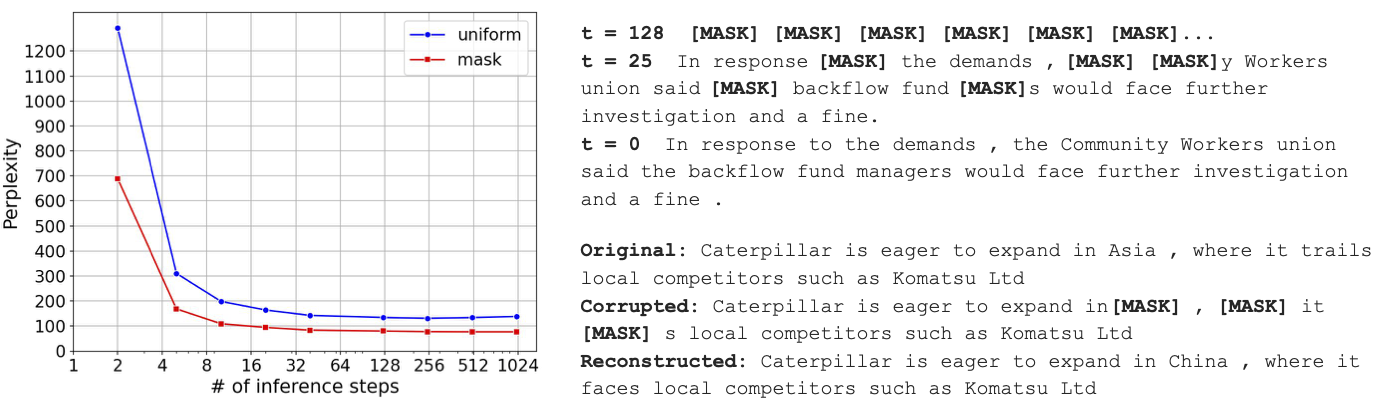
\includegraphics[width=\textwidth]{figures/perplexity3.png}
    \caption{Left: perplexity v.s. sampling iterations for LM1B. Right: Using a trained D3PM absorbing model for LM1B to (top) generate new sentences and (bottom) reconstruct corrupted examples.}
    \vspace{-0.3cm}
    \label{fig:lm1b_scaling}
\end{figure}
%

Table \ref{tab:lm1b} contains results from experiments on LM1B. Overall, mask diffusion (D3PM absorbing) does relatively well, approaching the performance of a comparable autoregressive model of the same size, and scaling to far fewer steps, while uniform diffusion performs significantly worse. We find, surprisingly, that the D3PM NN model performs worse than the uniform model in terms of log likelihoods (although it demonstrates unique qualitative behavior). This suggests that word embedding similarity may not be a meaningful kind of locality in a diffusion process. We found the the $L_{\lambda=0.01}$ loss worked best for the mask absorbing model, but reduced performance for the other models. We note the surprising scaling in perplexity in Figure \ref{fig:lm1b_scaling}, achieving strong results with as few as 10 inference steps. We also show samples from our model and completions from corrupted samples.
\begin{table}[t] % Daniel: Strong opinion against inline tables. Top or bottom only.
\vspace{-0.3cm}
  \caption{Quantitative results on LM1B. Perplexity reported on the test set. Results are reported on two seeds. All models have context window length 128 and 12 layers unless otherwise noted. $^\dagger$Transformer XL is a 24 layer transformer. $^\ddagger$rounded for readability, see Appendix~\ref{appendix:lm1b_aux}.}
  \label{tab:lm1b}
  \scriptsize
  \centering
  \begin{tabular}{r rrr c rrr}
    \toprule
    Metric: &\multicolumn{3}{c}{Perplexity ($\downarrow$)}
    &&\multicolumn{3}{c}{Sample time$^\ddagger$ (s) ($\downarrow$)}\\
    \cmidrule{2-4}\cmidrule{6-8}
    inference steps: & $1000$
    & $128$
    & $64$
    &
    & $1000$
    & $128$
    & $64$\\
    \midrule
    D3PM uniform
    & 137.9 $\pm$ 2.1 & 139.2 $\pm$ 1.2 & 145.0 $\pm$ 1.2 &
    & 1.82 & 0.21 & 0.08 \\
    D3PM NN
    & 149.5 $\pm$ 1.3 & 158.6 $\pm$ 2.2 & 160.4 $\pm$ 1.2 &
    & 21.29 & 6.69 & 5.88 \\
    D3PM absorbing
    & 76.9 $\pm$ 2.3 & 80.1 $\pm$ 1.2 & 83.6 $\pm$ 6.1 &
    & 1.90 & 0.19 & 0.10 \\
    \midrule
    Transformer (ours)
    & - & 43.6 & - &
    & - & 0.26 & -\\
    Transformer XL \citep{transformer_xl}$^\dagger$
    & - & 21.8 & - &
    & - & - & -\\
    \bottomrule
  \end{tabular}
%   \begin{tabular}{lllll}
%     \toprule
%     % \multicolumn{2}{c}{Part}                   \\
%     % \cmidrule(r){1-2}
%     Model & Perplexity @ 1000 steps & @ 128 steps & @ 64 steps & Sample time (at 1000/128/64)\\
%     \midrule
%     D3PM uniform \citep{hoogeboom2021argmax} (ours) & $159.85$ & $165.93$ & - & a/b/c \\
%     D3PM mask ($L_{\lambda=0.01}$) (ours) & $78.15\pm 4.1$ & $83.172$ & $89.13\pm 9.2$ & a/b/c \\
%     \midrule
%     Transformer decoder (ours) & - & $43.62549$ & - & -/b/- \\
%     Transformer XL \citep{transformer_xl}$^\dagger$ & - & $21.8$ & - & -/c/- \\
%     \bottomrule
%   \end{tabular}
\end{table}



\section{Image generation}

\begin{table}[t]
  \caption{Inception scores (IS), Frechet Inception Distance (FID) and negative log-likehood (NLL) on the image dataset CIFAR-10.  The NLL is reported on the test set in bits per dimension. We report our results as averages with standard deviations, obtained by training five models with different seeds.}
  \label{tab:cifar10}
  \scriptsize
  \centering
  \begin{tabular}{llll}
    \toprule
    \multicolumn{1}{l}{Model}  & IS ($\uparrow$)    & FID ($\downarrow$) & NLL ($\downarrow$)        \\
    \midrule
    Sparse Transformer \citep{child2019generating}    &        &       & 2.80\\
    NCSN  \citep{song_2019}                 & $8.87\pm0.12$ & 25.32  &\\
    NCSNv2  \citep{song2020improved}        & $8.40\pm0.07$ & 10.87  &\\
    StyleGAN2 + ADA  \citep{karras2020training}      & $9.74\pm0.05$ & 3.26 &\\
    \midrule
    Diffusion (original), $L_{\mathrm{vb}}$ \citep{sohl2015deep}  & & & $\leq 5.40$ \\
    DDPM $L_{\mathrm{vb}}$ \citep{ho2020denoising}  & $7.67 \pm 0.13$  &  $13.51$ & $\leq 3.70$  \\
    DDPM $L_{\mathrm{simple}}$ \citep{ho2020denoising} & $9.46 \pm 0.11$  &  $3.17$ & $\leq 3.75$ \\
    Improved DDPM $L_{\mathrm{vb}}$ \citep{nichol2021improved} &   & $11.47$ & $\leq 2.94$ \\
    Improved DDPM $L_{\mathrm{simple}}$ \citep{nichol2021improved} &   & $2.90$ & $\leq 3.37$ \\
    DDPM++ cont \citep{song2020_sde} &   &  $2.92$ & $2.99$ \\
    NCSN++ cont. \citep{song2020_sde}  & $9.89$ & $2.20$ & \\
    \midrule
    D3PM uniform $L_{\mathrm{vb}}$ & $5.99 \pm 0.14$  &  $51.27 \pm 2.15$ & $\leq 5.08 \pm 0.02$  \\
    D3PM absorbing $L_{\mathrm{vb}}$ & $6.26 \pm 0.10$  &  $41.28 \pm 0.65$ & $\leq 4.83 \pm 0.02$  \\
    D3PM absorbing $L_{\lambda=0.001}$  & $6.78 \pm 0.08$  &  $30.97 \pm 0.64$ & $\leq 4.40 \pm 0.02$ \\
    D3PM Gauss $L_{\mathrm{vb}}$ & $7.75 \pm 0.13$  &  $15.30 \pm 0.55$ & $\leq 3.966 \pm 0.005$  \\
    D3PM Gauss  $L_{\lambda=0.001}$ & $8.54 \pm 0.12$  &  $8.34 \pm 0.10$ & $\leq 3.975 \pm 0.006$ \\
    D3PM Gauss + logistic $L_{\lambda=0.001}$ & $8.56 \pm 0.10$  &  $7.34 \pm 0.19$ &  $\leq 3.435 \pm 0.007$ \\
    \bottomrule
  \end{tabular}
\end{table}


We evaluate the performance of several D3PM models on the task of unconditional image generation with the dataset CIFAR-10 \citep{krizhevsky2009learning}. We follow \citet{ho2020denoising} and use $T=1000$ timesteps for all models and verify that for all models the forward process converges to the stationary distribution within $T$ steps, yielding a value of at most $L_T\approx 10^{-5}$ bits per dimension. We train three versions of D3PM with different transition matrices: doubly stochastic matrices with uniform transition probabilities (D3PM uniform) \citep{hoogeboom2021argmax}, transition matrices with an absorbing state located at R, G and B values of 128 (D3PM absorbing) and doubly stochastic discretized Gaussian transition matrices (D3PM Gauss). For the D3PM uniform model we experimented with a linear $\beta_t$ schedule as well as the cosine schedule as proposed in \citep{hoogeboom2021argmax}, with the cosine schedule producing the best results. For D3PM absorbing we use the schedule $\beta_t = (T-t+1)^{-1}$ as also proposed in \citep{sohl2015deep}, which corresponds to increasing the probability of being in the absorbing state linearly over time.
For D3PM Gauss we use the same linear schedule as in \citep{ho2020denoising}. See Appendix \ref{sec:appendix_image} for more details on the experimental setup.

\begin{figure}[b]
    \centering
    \begin{subfigure}[b]{0.54\textwidth}
         \centering
         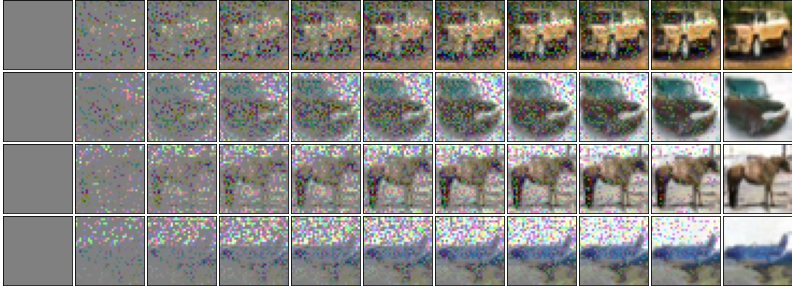
\includegraphics[width=\textwidth]{figures/progressive_samples_mask_hybrid.png} \\
         \vspace{0.07cm}
         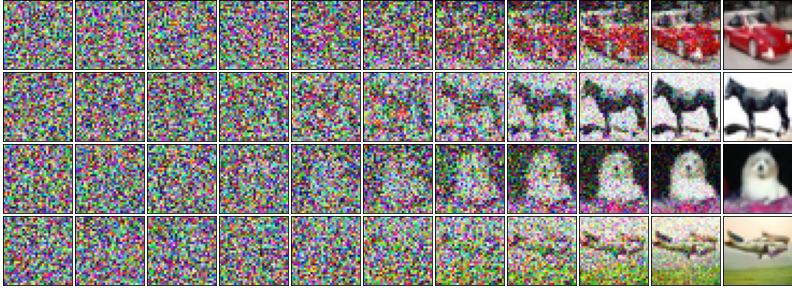
\includegraphics[width=\textwidth]{figures/progressive_samples_gauss_logistic_hybrid.png} 
     \end{subfigure}
     \hfill
     \begin{subfigure}[b]{0.45\textwidth}
         \centering
         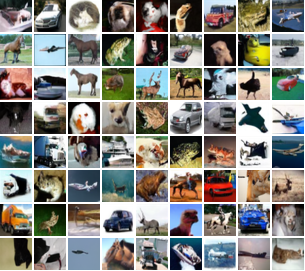
\includegraphics[width=\textwidth]{figures/cifar10_samples_cropped.png}
     \end{subfigure}
    \caption{Left: progressive sampling at $t=1000, 900, 800, ..., 0$ for D3PM absorbing (top) and D3PM Gauss + logistic (bottom), trained with $L_{\lambda}$ loss on CIFAR-10. These samples were cherry picked. Right: (non cherry picked) samples from the D3PM Gauss + logistic model.}
    \label{fig:cifar10_samples}
\end{figure}
Table~\ref{tab:cifar10} shows that for D3PM models trained with the $L_{\mathrm{vb}}$ objective, D3PM Gauss performs better than D3PM absorbing and uniform on all metrics: Inception score (IS), Frechet Inception Distance (FID) and negative log-likelihood (NLL). The IS score of the uniform and absorbing D3PM models are comparable, while the FID score and NLL of the D3PM absorbing model are slightly better. We trained both D3PM absorbing and D3PM Gauss with the alternative loss function $L_{\lambda}$ of \eqref{eq:alternative_loss}, and we found $\lambda=0.001$ to work best.
We have also experimented with larger values of $\lambda$ and a model trained only with the auxiliary denoising term in \eqref{eq:alternative_loss}. Although this led to a more rapid increase in performance early on in training, the NLL leveled off at higher values for larger $\lambda$ and the FID even started increasing again.
%}
The results show that the models trained with $L_{\lambda}$ perform significantly better than their counterparts trained with $L_{\mathrm{vb}}$.
%
One explanation for this boost in performance is that the cross entropy term leads to gradient noise that varies less with the time step $t$, which is in contrast to the large change in magnitude of the $L_{t-1}$ terms in $L_{\mathrm{vb}}$ for smaller $t$, as demonstrated by \citet{nichol2021improved}. 
Finally, we achieve our best results by combining D3PM Gauss trained on $L_{\lambda}$ with a truncated logistic parameterization of the reverse process distribution $p_{\theta}(\widetilde{\bx}_0|\bx_t)$ (D3PM Gauss + logistic). Figure~\ref{fig:cifar10_samples} shows samples from our best model (D3PM Gauss + logistic), as well as the D3PM absorbing model.

